\chapter{Estado de la cuestión}

\label{cap:estadoDeLaCuestion}
% En este apartado no tengo del todo claro qué contenido específico debería incluir, ya que existe cierta confusión con el capítulo siguiente, dedicado a la Descripción del Trabajo. Entiendo que aquí se debería reflejar el estado actual relacionado con el objeto de estudio, sin embargo, tiendo a mezclarlo con la investigación preliminar que realizamos, la cual corresponde a la fase inicial de la Descripción del Trabajo.
% En el estado de la cuestión es donde aparecen gran parte de las referencias bibliográficas del trabajo. Una de las formas más cómodas de gestionar la bibliografía en {\LaTeX} es utilizando \textbf{bibtex}. Las entradas bibliográficas deben estar en un fichero con extensión \textit{.bib} (con esta plantilla se proporciona el fichero biblio.bib, donde están las entradas referenciadas más abajo). Cada entrada bibliográfica tiene una clave que permite referenciarla desde cualquier parte del texto con los siguiente comandos:

% \begin{itemize}
% \item Referencia bibliografica con cite: \cite{ldesc2e}
% \item Referencia bibliográfica con citep: \citep{notsoshort}
% \item Referencia bibliográfica con citet: \citet{latexAPrimer}
% \end{itemize}

% Es posible citar más de una fuente, como por ejemplo \citep{latexCompanion,LaTeXLamport,texKnuth}

% Después, \LaTeX se ocupa de rellenar la sección de bibliografía con las entradas \textbf{que hayan sido citadas} (es decir, no con todas las entradas que hay en el .bib, sino sólo con aquellas que se hayan citado en alguna parte del texto).

% Bibtex es un programa separado de latex, pdflatex o cualquier otra cosa que se use para compilar los .tex, de manera que para que se rellene correctamente la sección de bibliografía es necesario compilar primero el trabajo (a veces es necesario compilarlo dos veces), compilar después con bibtex, y volver a compilar otra vez el trabajo (de nuevo, puede ser necesario compilarlo dos veces). 
\chapterquote{Somos sentimientos y tenemos seres humanos}{Rajoy}


La realidad aumentada (RA) se define como la superposición de información generada por computadora, como imágenes, vídeo o gráficos 3D, sobre el entorno real, con el objetivo de enriquecer la percepción del usuario y permitir la interacción en tiempo real \citep{Azuma1997}.  

A diferencia de la realidad virtual (RV), que sumerge completamente al usuario en un entorno simulado, la RA complementa la realidad existente sin sustituirla, manteniendo al usuario conectado con su entorno físico \citep{Billinghurst2015}.  

Las primeras aplicaciones de RA tuvieron un enfoque militar, como los sistemas HUD (head-up display) en aviones de combate, que proyectaban datos críticos sobre el campo visual del piloto sin bloquear su visión. Posteriormente, esta tecnología se adaptó a la aviación comercial y al sector automotriz, con HUDs que muestran instrucciones de navegación directamente sobre el campo visual del conductor \citep{Olsson2012}.  

En sus inicios, los componentes clave de un sistema de RA incluían un proyector para generar el contenido digital, un combinador que actuaba como superficie de proyección y un computador que procesaba los datos en tiempo real para integrarlos con el entorno físico \citep{Azuma1997}. Actualmente, la RA se implementa de manera mucho más accesible mediante dispositivos de uso cotidiano como smartphones y tablets, que aprovechan la cámara, los sensores integrados y la capacidad de procesamiento para ofrecer experiencias inmersivas.  

Los dispositivos más avanzados, como los HMDs (Head-Mounted Displays), emplean ópticas que superponen gráficos virtuales sobre la visión real. Para mantener la coherencia en la experiencia, incorporan sensores de seis grados de libertad (6DoF), lo que significa que son capaces de detectar tanto la traslación (movimiento en los tres ejes cartesianos) como la rotación (inclinación, giro y orientación) del usuario \citep{AzumaBishop1994}.  

A lo largo de su evolución, la RA ha pasado de depender de hardware especializado y costoso a integrarse en la vida diaria. Su presencia en aplicaciones como los filtros de redes sociales refleja un cambio fundamental: la tecnología se vuelve transparente y lo que prevalece es la experiencia aumentada.  

La RA en la actualidad se encuentra en un punto de madurez tecnológica que permite su aplicación en sectores muy diversos, como la medicina, la industria, la educación o el entretenimiento. Las grandes empresas tecnológicas han impulsado su integración en dispositivos de consumo masivo: Apple y Google han integrado ARKit \citep{ARKit} y ARCore \citep{ARCore} en sus ecosistemas móviles, lo que ha facilitado el desarrollo de aplicaciones accesibles y de gran impacto. La creciente capacidad de los dispositivos móviles y la popularización de herramientas de desarrollo están impulsando la creación de experiencias cada vez más complejas, interactivas y adaptadas a diferentes contextos. Esto convierte a la RA en una tecnología clave dentro de las tendencias actuales de comunicación digital e interacción inmersiva.

\section{Tipos de realidad aumentada}
\label{sec:tipos_ra}

La realidad aumentada (RA) es una tecnología muy versátil que no puede clasificarse mediante un único criterio, ya que sus aplicaciones y métodos de implementación varían ampliamente. Para entender sus distintas formas, se pueden considerar varios ejes de clasificación que ayudan a describir cómo funciona y cómo se percibe el contenido virtual en el mundo real.  

Un primer eje se centra en cómo el sistema determina la posición y orientación del contenido virtual dentro del entorno físico. En este caso, se distingue entre \textbf{RA basada en marcadores} (\textit{marker-based AR}), que utiliza patrones visuales predefinidos como códigos QR, imágenes o elementos físicos específicos para situar el objeto virtual, y \textbf{RA sin marcadores} (\textit{markerless AR}), que emplea sensores, visión por computador y técnicas como SLAM (Simultaneous Localization and Mapping) para comprender el entorno y colocar los objetos virtuales sin necesidad de marcadores explícitos.  

Un segundo eje se refiere a la forma en que se percibe la realidad y se combina con los elementos virtuales. En los sistemas \textbf{video see-through}, la realidad se observa a través de la cámara de un dispositivo (como un smartphone o tablet) y los elementos virtuales se dibujan sobre la imagen capturada. Por el contrario, en la \textbf{RA óptica} (\textit{optical see-through}) la imagen real se ve directamente a través de un cristal o lente, sobre el que se proyectan los gráficos virtuales, como ocurre en HUDs o en gafas inteligentes. Por último, en la \textbf{RA basada en proyección} (\textit{projection-based AR}) los elementos virtuales se proyectan directamente sobre superficies físicas, de manera que no se necesita una pantalla intermedia para percibir la combinación de realidad y contenido digital.  

Un tercer eje analiza la forma en que se integra el contenido virtual con el mundo real. En la \textbf{RA aditiva} (\textit{additive AR}) los objetos virtuales se suman a la escena real sin modificarla, simplemente enriqueciendo la información visual disponible. En cambio, en la \textbf{RA por superposición} (\textit{superimposition AR}) la vista de un objeto real puede ser reemplazada parcial o totalmente por su versión aumentada, lo que resulta útil en aplicaciones médicas, educativas o industriales donde es necesario sustituir o resaltar elementos específicos de la escena.  

Es importante destacar que estos ejes de clasificación no son excluyentes: una misma aplicación puede combinar características de varios criterios. Por ejemplo, un sistema puede ser markerless, usar superimposition AR y mostrarse mediante video see-through, mientras que otro podría combinar optical see-through con RA aditiva. Este enfoque multidimensional permite analizar con mayor precisión las capacidades y limitaciones de la RA, así como comprender mejor las posibilidades de implementación en diferentes contextos tecnológicos y de usuario.





La tabla~\ref{tabla:tiposRA} resume los principales tipos de RA con sus características técnicas y ejemplos de uso, lo que permite entender las distintas aproximaciones antes de analizar las herramientas disponibles para implementarlas.

\begin{table}[H]
\centering
\small
\begin{tabularx}{\textwidth}{l X X}
\toprule
\textbf{Tipo de RA} & \textbf{Mecanismo} & \textbf{Aplicaciones típicas} \\
\midrule
\textbf{Basada en marcadores} & Detecta un patrón visual predefinido (QR, imagen) para posicionar el objeto virtual. & Manuales técnicos, publicidad interactiva, tarjetas de visita. \\[4pt]
\textbf{Sin marcadores (SLAM)} & Reconstruye el entorno mediante cámara e IMU, sin referencia física explícita. & Pokémon GO, filtros de Instagram, decoración virtual. \\[4pt]
\textbf{Por proyección} & Proyecta imagen digital directamente sobre una superficie física. & Teclados virtuales, mesas interactivas, mapeo en arquitectura. \\[4pt]
\textbf{Por superposición} & Reemplaza parcial o totalmente la vista de un objeto por su versión aumentada. & Formación médica, mantenimiento industrial, cirugía asistida. \\
\bottomrule
\end{tabularx}
\caption{Comparativa de tipos de Realidad Aumentada}
\label{tabla:tiposRA}
\end{table}



\section{Aplicaciones de la Realidad Aumentada}
\label{sec:aplicaciones_ra}

La Realidad Aumentada ha dejado de ser una tecnología de nicho para convertirse en una herramienta de uso generalizado en múltiples industrias. Grand View Research valoró el mercado global de la RA en unos 70,2 mil millones de dólares en 2023, con una trayectoria de crecimiento sostenido impulsada por la madurez de los dispositivos de consumo y la proliferación de smartphones con capacidades de visión por computador \citep{GrandViewAR}. El despliegue de redes 5G está acelerando adicionalmente esta tendencia, al reducir la latencia y aumentar el ancho de banda disponible para aplicaciones inmersivas en tiempo real \citep{Ericsson_2020}. A continuación se presentan los ámbitos de aplicación más representativos de esta tecnología.

Las aplicaciones de la RA son amplias y variadas:
\begin{itemize}
    \item \textbf{Eventos en Vivo:} Un ejemplo destacado es el uso de RA durante el Super Bowl LIX, donde Fox Sports superponía en tiempo real gráficos, estadísticas y animaciones directamente sobre la imagen en vivo, enriqueciendo la comprensión del juego y la inmersión del espectador \cite{SportsVideo2025}. En la sección~\ref{sec:obs_studio} se analiza en detalle cómo se construye técnicamente una escena de este tipo dentro de OBS Studio.


    \item \textbf{Noticias:} En una pieza sobre las elecciones en Estados Unidos, el presentador Carlos Franganillo apareció teletransportado a escenarios como la Convención de Filadelfia o la Capilla Sixtina usando RA, lo que permitió explicar en directo el proceso de votación con desplazamientos y visualizaciones inmersivas \citep{Panorama2024}.

\begin{figure}[H]
  \centering
  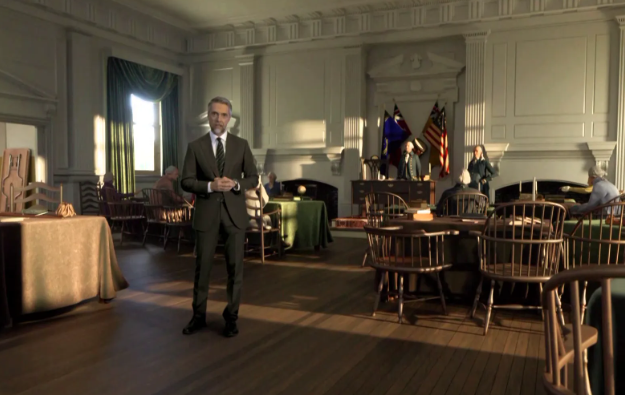
\includegraphics[height=2.5in]{Imagenes/Vectorial/noticias.png}
  \caption{Aplicación de la realidad aumentada (RA) en informativos televisivos para la visualización de datos y escenarios virtuales.}
  \label{fig:ra-noticias}
\end{figure}


   
    \item \textbf{Entretenimiento y Redes Sociales:} Los filtros de Realidad Aumentada (RA) y las pruebas virtuales (como probarse ropa o accesorios) se han convertido en herramientas fundamentales en plataformas como Snapchat, Instagram y TikTok. Según Snap Inc., un alto porcentaje de usuarios de la Generación Z utiliza filtros y lentes AR para probar virtualmente productos antes de tomar una decisión de compra, aumentando la confianza del consumidor y la conexión emocional con las marcas \citep{SnapchatGenZ2022}. Desde la perspectiva del impacto en negocio, BrandXR \citep{BrandXR2025}, empresa especializada en RA, estima que el 92\% de los usuarios que interactúan con contenido AR en estas plataformas realizan alguna acción posterior (compartir, visitar una web o completar una compra), lo que indica un vínculo directo entre la experiencia aumentada y el comportamiento del usuario. Las transmisiones en vivo en Instagram Live y Facebook Live han incorporado también elementos de RA para enriquecer actuaciones de artistas y la promoción de productos, creando un entorno multimedia especialmente atractivo para audiencias jóvenes.
\begin{figure}[H]
  \centering
  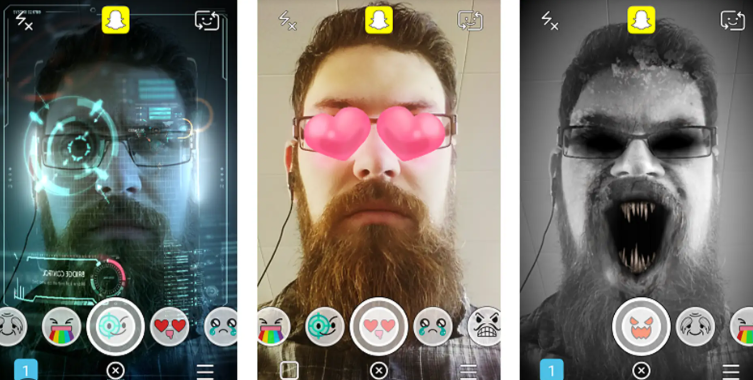
\includegraphics[height=2.5in]{Imagenes/Vectorial/rrss.png}
  \caption{Ejemplo de filtro con realidad aumentada (RA) en la red social Snapchat, utilizado para superponer elementos virtuales sobre el rostro del usuario en tiempo real.}
  \label{fig:filtro-snapchat}
\end{figure}


    \item \textbf{Esports:} La Realidad Aumentada está transformando la forma en que se transmiten los esports. Plataformas como ESTV integran gráficos AR en transmisiones en vivo, aportando visualizaciones interactivas sobre el presentador y estadísticas del juego que mejoran la narrativa del match \citep{ESTV2022}.
\begin{figure}[H]
  \centering
  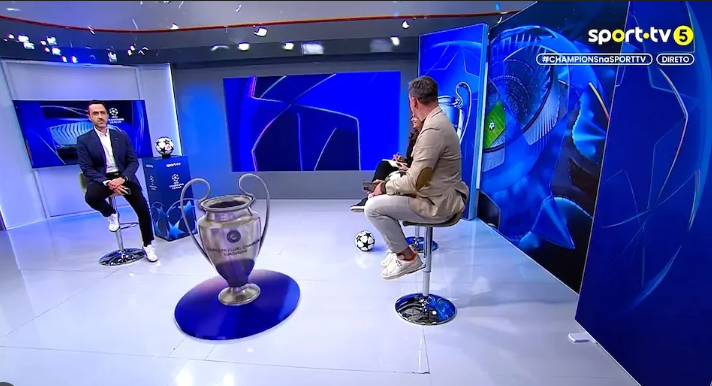
\includegraphics[height=2.5in]{Imagenes/Vectorial/sports.png}
  \caption{Uso de la realidad aumentada (RA) en retransmisiones en vivo de competiciones de \textit{eSports}, donde se integran elementos virtuales en la escena para mejorar la visualización y el análisis del evento.}
  \label{fig:ra-esports}
\end{figure}


    \item \textbf{Educación:} La Realidad Aumentada fusiona el entorno físico del estudiante con contenido virtual, ofreciendo experiencias interactivas que mejoran la retención y comprensión de conceptos complejos. Las revisiones sobre tecnologías inmersivas en educación superior constatan que estas herramientas favorecen el aprendizaje activo y mejoran la comprensión de contenidos abstractos \citep{Radianti2020}. En concreto, la RA resulta especialmente valiosa en disciplinas como la medicina, donde permite visualizar modelos anatómicos tridimensionales de forma interactiva, o en ingeniería y ciencias, donde facilita la comprensión espacial de fenómenos difíciles de representar en dos dimensiones. Estas aplicaciones son efectivas desde la educación primaria hasta el nivel universitario.
\begin{figure}[H]
  \centering
  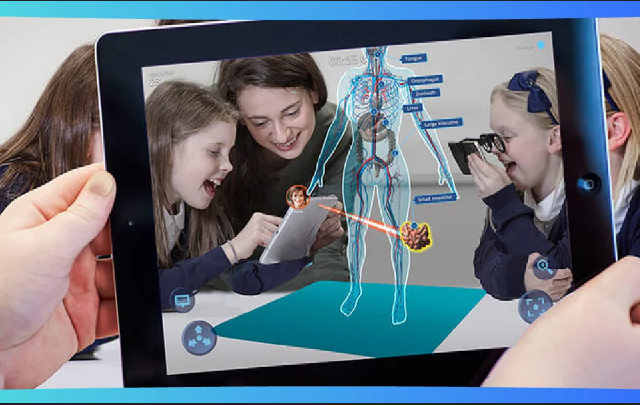
\includegraphics[height=2.5in]{Imagenes/Vectorial/education.png}
  \caption{Ejemplo de aplicación de la realidad aumentada (RA) en el ámbito educativo, utilizada para el aprendizaje de anatomía y procedimientos médicos mediante la visualización interactiva de modelos tridimensionales.}
  \label{fig:ra-medicina}
\end{figure}

\end{itemize}

La diversidad de aplicaciones descrita en esta sección evidencia que la RA necesita apoyarse en herramientas de desarrollo maduras. En la siguiente sección se analizan los principales SDKs y bibliotecas disponibles para implementar RA en tiempo real, con el objetivo de seleccionar la más adecuada para este proyecto.

\section{APIs y SDKs de Realidad Aumentada}
\label{sec:apis_ra}

Antes de abordar la integración de experiencias de Realidad Aumentada (RA) en aplicaciones prácticas, es importante describir de forma clara y separada las capacidades y limitaciones de las principales bibliotecas y SDKs disponibles en este campo.

\subsection{Vuforia}
\label{subsec:vuforia}

Vuforia \citep{Vuforia} es uno de los Software Development Kits (SDK) más consolidados en el ámbito de la RA. Desarrollado originalmente por Qualcomm y actualmente mantenido por PTC Inc., está orientado al reconocimiento y seguimiento de imágenes, objetos y entornos en tiempo real. Su principal objetivo es facilitar la integración de experiencias de RA en aplicaciones móviles y de escritorio, con un énfasis especial en la compatibilidad con el motor de videojuegos Unity.

Una de las características distintivas de Vuforia es su robustez en el seguimiento visual. El SDK permite detectar y rastrear múltiples tipos de elementos: desde imágenes planas (\textit{Image Targets}) hasta objetos tridimensionales, cilindros o incluso entornos más complejos mediante \textit{Model Targets}. Para gestionar estos elementos, ofrece un sistema de creación de bases de datos de marcadores (\textit{Target Manager}), que simplifica la preparación de activos para ser usados dentro de proyectos de RA.

\textbf{Entre sus principales ventajas} se encuentra la integración profunda con Unity, que no solo proporciona librerías y prefabs listos para usar, sino también un flujo de trabajo optimizado para importar, configurar y desplegar elementos de realidad aumentada. Además, Vuforia ofrece funcionalidades avanzadas como reconocimiento de texto, detección de planos y soporte para experiencias multiusuario.

\textbf{En cuanto a sus limitaciones}, Vuforia presenta un modelo de licenciamiento que restringe ciertas funcionalidades en proyectos comerciales. Asimismo, aunque dispone de soporte para desarrollo en C++ y aplicaciones nativas, su orientación principal hacia Unity y dispositivos móviles lo aleja de ser un SDK completamente flexible para aplicaciones de escritorio más especializadas.

\textbf{En resumen}, Vuforia se posiciona como una solución madura y ampliamente adoptada para proyectos de RA en entornos móviles y en el ecosistema Unity. Su facilidad de uso y robustez lo hacen ideal para prototipado rápido y despliegue en aplicaciones comerciales, aunque sus restricciones de licencia lo diferencian de alternativas abiertas como ARToolKit o OpenCV.

\subsection{ARToolKit}
\label{subsec:artoolkit}

ARToolKit \citep{ARToolkit} es uno de los SDK más veteranos y representativos en el campo de la RA, ampliamente reconocido por haber introducido el tracking por marcadores como técnica fundamental en los primeros sistemas. Se trata de un software de código abierto, disponible con APIs en C y C++, y diseñado desde sus inicios con un enfoque multiplataforma. Su simplicidad conceptual y su carácter abierto lo han convertido en una herramienta muy utilizada en el ámbito académico y en proyectos de investigación.

La \textbf{principal aportación} de ARToolKit radica en la detección y el seguimiento de patrones visuales impresos (marcadores), que permiten calcular en tiempo real la posición y orientación de la cámara respecto a ellos.

\textbf{Entre sus ventajas}, destaca la licencia libre que elimina restricciones comerciales y facilita su adopción en proyectos experimentales. También proporciona un control granular sobre el pipeline de visión, ya que el desarrollador puede modificar o extender directamente el código fuente. Esto lo convierte en una opción idónea para prototipos rápidos, entornos académicos y proyectos de investigación.

\textbf{En cuanto a limitaciones}, ARToolKit requiere un mayor esfuerzo de integración en comparación con SDKs comerciales como Vuforia, pues no ofrece flujos de trabajo optimizados ni integración directa con motores gráficos modernos. Además, su enfoque centrado en el uso de marcadores lo hace menos versátil frente a soluciones actuales que incorporan detección de objetos, planos o entornos completos. La calibración manual de cámaras es también un requisito frecuente para alcanzar un rendimiento óptimo.

\subsection{OpenCV}
\label{subsec:opencv}

OpenCV \citep{OpenCV} es una biblioteca de visión por computador de código abierto, ampliamente utilizada en el procesamiento de imágenes y vídeo en tiempo real. Aunque no es un SDK de RA completo, proporciona un conjunto muy extenso de algoritmos y utilidades que permiten construir soluciones de RA de manera modular y personalizada.

La \textbf{principal aportación} de OpenCV consiste en sus herramientas para la detección de características visuales, la estimación de pose y el procesamiento eficiente de flujos de vídeo, lo que lo convierte en un recurso fundamental para implementar sistemas de tracking y análisis visual sobre los que se pueden superponer contenidos sintéticos.

\textbf{Entre sus ventajas}, destaca su carácter abierto y gratuito, la gran comunidad de desarrolladores que asegura mantenimiento y documentación abundante, así como su disponibilidad multiplataforma. Además, ofrece gran flexibilidad para integrar algoritmos propios y optimizar el rendimiento en función de las necesidades específicas del proyecto.

\textbf{En cuanto a limitaciones}, OpenCV no ofrece directamente un sistema de tracking listo para producción ni incluye componentes gráficos o de gestión de activos de RA. Su uso exige un esfuerzo adicional de desarrollo, incluyendo la calibración de cámaras, la integración con GPU si se requiere alto rendimiento, y la implementación de capas adicionales para generar experiencias completas de RA.

\subsection{SDKs de NVIDIA}
\label{subsec:nvidia_sdk}

Los SDKs de NVIDIA, entre los que destacan Maxine y diversas librerías de inferencia aceleradas por GPU \citep{SDK_NVIDIA}, proporcionan un conjunto de herramientas orientadas al procesamiento visual mediante inteligencia artificial. Estos SDKs están optimizados para aprovechar los Tensor Cores de las tarjetas gráficas RTX, ofreciendo un alto rendimiento en tareas intensivas como el seguimiento facial, la detección de puntos clave o la segmentación de vídeo.

La \textbf{principal aportación} de los SDKs de NVIDIA consiste en permitir el uso de modelos de visión por computador e IA en tiempo real con baja latencia. Su enfoque se centra especialmente en aplicaciones de análisis facial y manipulación de vídeo asistida por inteligencia artificial.

\textbf{Entre sus ventajas}, destacan la precisión y velocidad de sus algoritmos, el soporte para tareas avanzadas como reconstrucción facial 3D o sustitución de fondo, y la integración con frameworks de desarrollo actuales.

\textbf{En cuanto a limitaciones}, el uso de estos SDKs está restringido a sistemas con hardware compatible (GPUs NVIDIA RTX), lo que limita su accesibilidad en entornos heterogéneos. Además, presentan diferencias en soporte multiplataforma: ciertos SDKs, como Maxine, tienen compatibilidad reducida en Linux en comparación con Windows. A ello se suman las restricciones de licencia y distribución que condicionan su utilización en proyectos comerciales, lo que los diferencia de alternativas abiertas como OpenCV o ARToolKit.

\subsection{DeepAR}
\label{subsec:deepar}

DeepAR \citep{DeepAR} es un SDK orientado específicamente a la generación de efectos faciales en tiempo real, ofreciendo funcionalidades como maquillaje virtual, embellecimiento automático, aplicación de filtros visuales y reemplazo de fondo. A diferencia de bibliotecas más generales, su propuesta se centra en proporcionar un conjunto de herramientas listas para usar, acompañadas de una amplia colección de assets predefinidos.

La \textbf{principal aportación} de DeepAR radica en simplificar el desarrollo de aplicaciones con efectos visuales sobre rostros, reduciendo el tiempo de implementación mediante librerías optimizadas y recursos gráficos integrados.

\textbf{Entre sus ventajas}, destacan la facilidad de integración, la disponibilidad de efectos listos para producción y el enfoque directo a experiencias de RA aplicadas a presentadores o participantes en contextos interactivos. Esto permite obtener resultados rápidos sin necesidad de diseñar desde cero el pipeline de visión o los modelos faciales.

\textbf{En cuanto a limitaciones}, el SDK mantiene un enfoque centrado en rostros, por lo que resulta menos adecuado para tareas de RA que requieran seguimiento de objetos, planos o entornos completos. Además, se distribuye bajo un modelo comercial de licenciamiento, lo cual restringe su uso gratuito a fases de prueba o prototipado y puede implicar costes adicionales en proyectos de producción.

\subsection{Comparativa de todas las herramientas}
\label{subsec:comparativa-sdks}
\begin{table}[H]
\centering
\small % Fuente más pequeña
\begin{tabularx}{\textwidth}{X X X} % X hace que las columnas se ajusten al ancho
\toprule
\textbf{SDK/Biblioteca} & \textbf{Características} & \textbf{Plataformas} \\
\midrule
Vuforia  & Seguimiento de imágenes y objetos 3D & Multiplataforma \\
ARToolkit & Seguimiento basado en marcadores & Multiplataforma \\
OpenCV  & Detección y seguimiento de objetos & Multiplataforma \\
NVIDIA  & Seguimiento facial avanzado & Windows \\
DeepAR  & Filtros faciales 3D & Web, Android, iOS, Desktop \\
\bottomrule
\end{tabularx}
\caption{Comparativa de SDKs y bibliotecas de RA}
\label{tab:comparativa-sdks}
\end{table}
\subsection{Decisión tecnológica: OpenCV y el módulo ArUco}
\label{subsec:decision_tecnologica}

De los SDK y bibliotecas analizados, la elección para este trabajo recayó sobre \textbf{OpenCV} junto con su módulo de detección de marcadores fiduciarios \textbf{ArUco} \citep{GarridoJurado2014}. Esta decisión se sustenta en cuatro criterios concretos derivados de los requisitos del sistema.

En primer lugar, la \textbf{licencia Apache~2.0} de OpenCV elimina cualquier restricción de distribución del plugin, a diferencia de Vuforia o DeepAR, que requieren licencias comerciales para uso en producción. En segundo lugar, OpenCV ofrece una \textbf{API nativa en C++} basada en funciones puras, sin dependencias de motores gráficos como Unity, lo que permite enlazarlo como biblioteca estática dentro del plugin de OBS sin conflictos de ABI. En tercer lugar, el módulo ArUco implementa el algoritmo \textbf{PnP} (\textit{Perspective-n-Point}) para la estimación de pose en tiempo real a partir de los cuatro vértices del marcador, devolviendo directamente el vector de rotación y el vector de traslación de la cámara con precisión suficiente para anclar objetos 3D sobre vídeo HD \citep{GarridoJurado2014}. En cuarto lugar, OpenCV incluye las herramientas de \textbf{calibración de cámara} necesarias para corregir la distorsión óptica de cada objetivo (un requisito previo para que la estimación de pose sea métricamente correcta), integradas en la misma biblioteca, sin dependencias adicionales.

ARToolKit habría podido cubrir un rol similar en lo referente al tracking por marcadores, pero su ecosistema de desarrollo es menos activo y su módulo de estimación de pose no alcanza la madurez ni el soporte de la comunidad que ofrece OpenCV. Los SDKs de NVIDIA y DeepAR se descartan por requerir hardware específico y licencias privativas, respectivamente, y Vuforia por su orientación a Unity y su modelo de licenciamiento restrictivo para plugins de terceros.

\section{OBS Studio}
\label{sec:obs_studio}

Las aplicaciones de Realidad Aumentada descritas en la sección anterior comparten un requisito común: necesitan un software que capture, componga y emita vídeo en tiempo real. En el ámbito de la retransmisión en vivo, OBS Studio \cite{OBS} es la plataforma de referencia, ya que combina la gratuidad, la compatibilidad multiplataforma y una arquitectura abierta que permite añadirle funcionalidades mediante plugins sin modificar su núcleo. Es precisamente esta extensibilidad la que hace de OBS Studio el entorno idóneo para desarrollar un plugin de RA en tiempo real.

OBS Studio es un software libre y de código abierto para la grabación de vídeo y la transmisión en vivo. Funciona como una mesa de mezclas audiovisual digital que combina fuentes de diversa naturaleza (pantalla, aplicaciones, cámaras, archivos multimedia) en escenas que pueden emitirse en directo o grabarse localmente. Su arquitectura modular permite integrar múltiples fuentes de audio y vídeo, realizar transiciones dinámicas entre escenas y aplicar filtros y efectos en tiempo real.

\subsection{OBS Studio como usuario}
\label{subsec:obs_usuario}

Para entender cómo OBS Studio organiza el vídeo, conviene distinguir con claridad sus dos conceptos fundamentales: la \textbf{escena} y la \textbf{fuente}. Una \textbf{escena} es el resultado final que se emite: el lienzo completo que el espectador ve. Ese lienzo se construye apilando \textbf{fuentes}, que son los elementos individuales que aportan contenido visual o sonoro. Cada fuente es independiente y puede colocarse, redimensionarse y ordenarse dentro de la escena. La diferencia clave es que la \textbf{escena define qué se emite}, mientras que las \textbf{fuentes definen de dónde procede cada elemento}. Los \textbf{filtros} operan sobre una fuente concreta y modifican su imagen antes de que se incorpore al lienzo: un filtro de croma, por ejemplo, elimina el color verde de una cámara antes de mezclarla con el fondo. Los filtros no son visibles por sí solos, siempre actúan sobre una fuente. Finalmente, las \textbf{transiciones} controlan la animación que ocurre cuando el operador cambia de una escena a otra, y el \textbf{mezclador de audio} gestiona el volumen y los efectos de sonido de todas las fuentes de forma centralizada.

La figura~\ref{fig:obs-ui} muestra OBS Studio durante una sesión de composición real. En la ventana de previsualización central se ve el resultado de combinar varias fuentes activas en la misma escena. En la zona inferior de la interfaz aparecen listadas las fuentes que la componen, cada una con su nombre y tipo, junto con el mezclador de audio. El panel lateral recoge los controles de retransmisión y grabación. Cada fuente puede tener sus propios filtros configurados, que OBS aplica de forma independiente antes de incorporar esa fuente al lienzo final.

\begin{figure}[H]
  \centering
  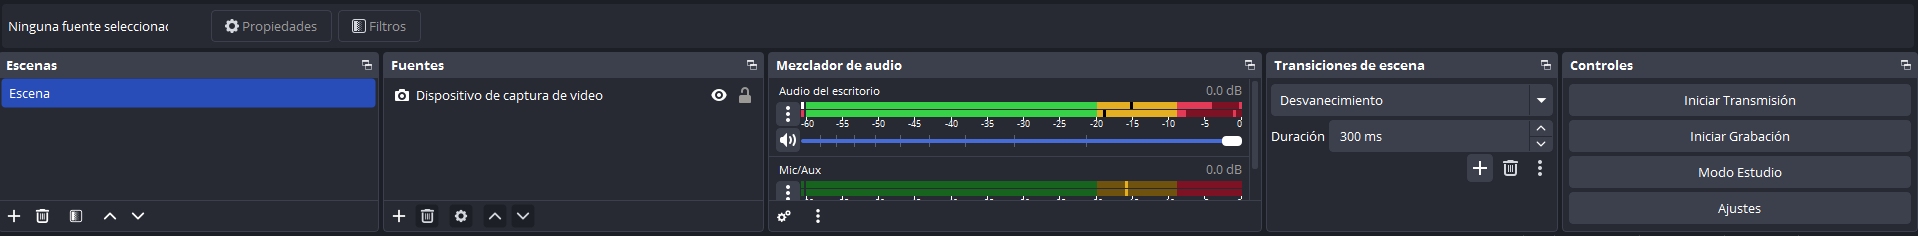
\includegraphics[width=\textwidth]{Imagenes/Vectorial/obsUI.png}
  \caption{Interfaz de OBS Studio mostrando una sesión de composición real con múltiples fuentes activas, filtros configurados y el panel de control de la retransmisión.}
  \label{fig:obs-ui}
\end{figure}

A continuación se describen estos componentes con más detalle:

\begin{itemize}
    \item \textbf{Escenas:} Son la unidad principal de organización en OBS. Cada escena combina múltiples fuentes de audio y vídeo en una composición completa que puede emitirse en directo. Se pueden crear escenas ilimitadas y cambiar entre ellas mediante transiciones predefinidas o personalizadas.

    \item \textbf{Fuentes:} Son los elementos individuales que aportan contenido a una escena. Entre las categorías más comunes se incluyen la captura de pantalla o ventana, el dispositivo de captura de vídeo (cámaras web), archivos multimedia, navegador web (contenido HTML/CSS/JavaScript), texto estático o dinámico, y una aplicación externa operando como cámara virtual (por ejemplo, Unreal Engine o Unity), lo que permite integrar el resultado de un pipeline de renderizado externo sin modificar el núcleo de OBS.

    \item \textbf{Filtros y efectos:} Operan sobre una fuente concreta y modifican su imagen antes de que se incorpore al lienzo. Entre los filtros de vídeo más habituales están la corrección de color, el croma, el recorte y el desenfoque; entre los de audio, la reducción de ruido y la ecualización. Los \textbf{filtros de vídeo son el punto de integración natural para un plugin de RA}: al actuar directamente sobre los frames de la cámara antes de que OBS los componga, el plugin puede detectar marcadores y renderizar geometría 3D en el mismo ciclo de procesamiento, sin duplicar la fuente ni introducir intermediarios.

    \item \textbf{Transiciones:} Animaciones que suavizan el paso de una escena a otra. OBS incluye transiciones predeterminadas y permite añadir nuevas mediante plugins.

    \item \textbf{Mezclador de audio:} Gestiona el volumen de cada fuente de audio, permite aplicar filtros y sincroniza el audio con el vídeo.
\end{itemize}

Para ilustrar cómo se articulan estos componentes en un caso real, la figura~\ref{fig:superbowl-obs} muestra la retransmisión del Super Bowl LIX de Fox Sports \citep{SportsVideo2025}, una de las producciones en vivo con mayor complejidad técnica del mundo. Desde la perspectiva de OBS, una escena de este tipo se construye apilando varias fuentes independientes a las que se aplican filtros antes de componer la imagen final.

\begin{figure}[H]
  \centering
  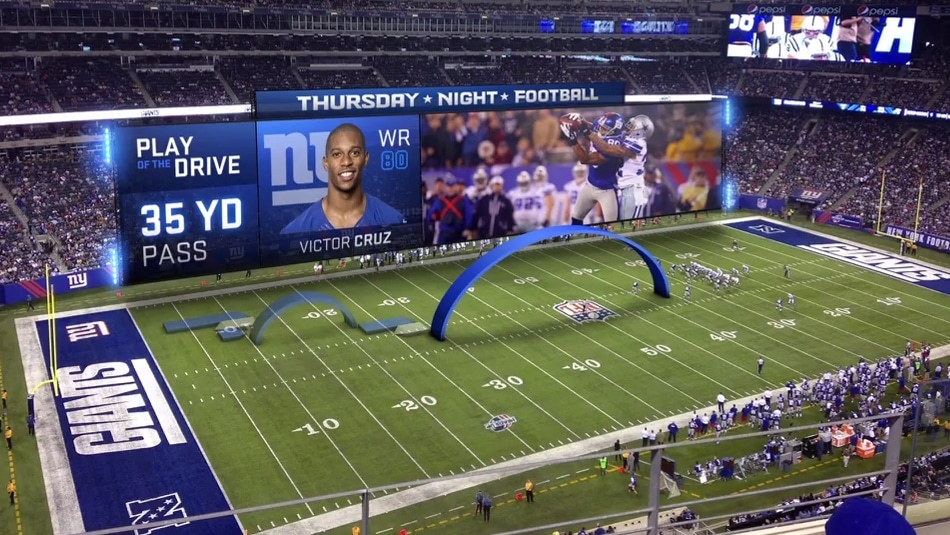
\includegraphics[width=\textwidth]{Imagenes/Vectorial/Eventosenvivo.jpg}
  \caption{Retransmisión del Super Bowl LIX por Fox Sports, donde se combinan la señal de cámara del estadio, el score bug y los gráficos de RA en una única escena compuesta.}
  \label{fig:superbowl-obs}
\end{figure}

\begin{itemize}
  \item \textbf{Fuente principal (cámara del estadio):} la señal de la cámara broadcast se incorpora a OBS como primera fuente de la escena, ocupando el lienzo completo y sirviendo de fondo de la composición. Sobre esta fuente se aplica un \textbf{filtro de corrección de color} para ajustar la temperatura, la exposición y el contraste según las condiciones lumínicas del estadio.
  \item \textbf{Fuente de overlay, score bug y estadísticas:} el \textit{score bug} (panel gráfico de puntuación superpuesto en la esquina de la imagen, estándar en retransmisiones deportivas) que se aprecia en la figura~\ref{fig:superbowl-obs}, con los logos de los dos equipos, el marcador y el reloj del partido, es un elemento gráfico independiente generado por un motor de gráficos broadcast y entregado a OBS como fuente de cámara virtual o como fuente de navegador.
  \item \textbf{Fuente de overlay, gráficos de RA:} los elementos sobreimpresos en el campo, como la línea de primera bajada, los puntos de seguimiento de jugadores y las estadísticas flotantes, son producidos por una aplicación externa especializada y entregados a OBS como cámara virtual con canal alfa. Al incorporar transparencia, OBS los compone directamente sobre la imagen del campo sin modificar el fondo.
\end{itemize}

La figura~\ref{fig:obs-layers-superbowl} muestra cómo se organizan estas capas dentro de OBS para producir la imagen final.

\begin{figure}[H]
\centering
\begin{tikzpicture}[
  B/.style={draw, rounded corners=3pt, minimum width=9cm, minimum height=1.2cm,
            font=\small, align=center, inner sep=7pt, text width=8.4cm},
  R/.style={draw=green!55!black, thick, rounded corners=3pt, minimum width=9cm,
            minimum height=0.85cm, fill=green!10, font=\small\bfseries, align=center},
  arr/.style={-Stealth, thick, gray!75}
]

\node[B, fill=blue!10]   (c3) at (0, 4.0)
  {\textbf{Capa 3 — Gráficos de RA} {\small (canal alfa)}\\[3pt]
   {\scriptsize\color{gray!80} línea de primera bajada · estadísticas flotantes · seguimiento de jugadores}};

\node[B, fill=orange!10] (c2) at (0, 2.1)
  {\textbf{Capa 2 — Score bug y estadísticas}\\[3pt]
   {\scriptsize\color{gray!80} logos de equipo · marcador · reloj del partido}};

\node[B, fill=gray!12]   (c1) at (0, 0.2)
  {\textbf{Capa 1 — Señal de cámara del estadio}\\[3pt]
   {\scriptsize\color{gray!80} imagen en vivo del campo · fondo completo de la escena}};

\draw[arr] (c1.north) -- (c2.south);
\draw[arr] (c2.north) -- (c3.south);

\draw[arr] (0, -0.55) -- (0, -1.22)
  node[midway, right=5pt, font=\scriptsize\itshape, gray] {composición en OBS};

\node[R] at (0, -1.68) {Imagen final emitida};

\end{tikzpicture}
\caption{Composición en capas de la escena OBS en la retransmisión del Super Bowl LIX (Fox Sports): tres fuentes independientes que OBS combina en la imagen final.}
\label{fig:obs-layers-superbowl}
\end{figure}

La posibilidad de incorporar aplicaciones externas como fuente resulta especialmente relevante en el contexto de la realidad aumentada. Un motor gráfico externo puede encargarse del pipeline de RA y entregar su resultado a OBS como si fuese una cámara virtual, sin necesidad de modificar OBS en absoluto. Esta estrategia, junto con la alternativa nativa mediante plugin, se analiza en detalle en la sección~\ref{sec:integracion_obs}.

\subsection{Desarrollo de plugins}
\label{subsec:desarrollo_plugins}

La arquitectura de escenas, fuentes y filtros descrita en el apartado anterior es extensible. OBS Studio permite que desarrolladores externos añadan nuevos tipos de fuentes y filtros mediante \textbf{plugins}. Desde el punto de vista del usuario, un plugin es simplemente una biblioteca que OBS carga al inicio y que amplía el menú de componentes disponibles. Desde el punto de vista técnico, es una extensión que se enlaza a la API pública de OBS y puede declarar nuevas fuentes, filtros y comportamientos gráficos, integrándose de forma transparente con el resto del sistema.

Esta capacidad de extensión es la que sustenta el trabajo de este TFG. El objetivo es desarrollar exactamente uno de estos plugins: un componente nativo de OBS capaz de consultar en tiempo real la API del sistema de jurado de un concurso de programación y superponer la información resultante sobre la imagen de la cámara. Entender la anatomía, el despliegue y las decisiones de diseño de un plugin de OBS es, por tanto, el paso previo necesario para abordar ese desarrollo.
 
\subsubsection*{Anatomía de un plugin}

Desde la perspectiva técnica, un plugin para OBS Studio es un paquete de herramientas con responsabilidades  diferenciadas. Es relevante  describir los tipos de archivos que suelen componerlo y la función que desempeña cada uno para un futuro desarrollo:

\begin{itemize}
  \item \textbf{Binario principal:} la biblioteca compilada (\texttt{.dll}, \texttt{.so} o \texttt{.dylib}) que contiene el código nativo del plugin. Este artefacto exporta las funciones que OBS invoca para registrar y gestionar las fuentes o filtros que el plugin proporciona.
  \item \textbf{Manifest / descriptor:} fichero que documenta metadatos del plugin (nombre, versión, autor, dependencias opcionales, etc.). Aunque OBS no exige un manifiesto complejo, un descriptor estructurado facilita la instalación, diagnóstico y mantenimiento.
  \item \textbf{Recursos gráficos y auxiliares:} shaders, texturas, modelos, iconos y otros activos necesarios en tiempo de ejecución. Estos archivos deben organizarse de forma coherente para permitir su localización y posibles traducciones.
  \item \textbf{Archivos de configuración:} ficheros JSON, INI o similares que almacenan parámetros por defecto, rutas relativas o presets. Permiten personalizar el comportamiento del plugin sin tocar el binario.
  \item \textbf{Scripts y utilidades auxiliares:} en algunos casos se incluyen scripts de ayuda (por ejemplo para pruebas, generación de assets o herramientas de conversión). Pueden estar escritos en Lua, Python o como simples scripts de shell/batch.
  \item \textbf{Documentación y licencias:} README, changelog y archivos de licencia que ayudan a la distribución y uso responsable del plugin.
\end{itemize}



\subsubsection*{Despliegue y rutas en OBS Studio}

El despliegue define dónde coloca el usuario u OBS los archivos del plugin y cómo OBS los detecta al iniciar. Las convenciones siguientes son las recomendadas en el ecosistema OBS:

\begin{itemize}
  \item \textbf{Carpeta de binarios:} los binarios compilados se colocan en \path{obs-plugins/arquitectura} dentro de la instalación de OBS (por ejemplo \path{obs-plugins/64bit/}). OBS explora estas rutas al arrancar y carga automáticamente las bibliotecas válidas.
  \item \textbf{Carpeta de datos:} los recursos adicionales deben residir en \path{data/obs-plugins/<nombre>/}. Aquí se ubican shaders, textos de localización, iconos y cualquier archivo que el plugin cargue en tiempo de ejecución mediante rutas relativas.


  \item \textbf{Rutas de usuario para desarrollo:} durante el desarrollo es habitual desplegar versiones en carpetas de usuario (sin privilegios de administrador) que OBS también revisa. Esto facilita pruebas iterativas sin afectar la instalación global.
  \item \textbf{Carga automática y reinicio:} OBS carga plugins al inicio, por lo que instalar, actualizar o eliminar un plugin normalmente requiere reiniciar la aplicación para que los cambios tomen efecto.
  \item \textbf{Permisos y empaquetado:} al distribuirse en entornos multiusuario o en máquinas con restricciones, hay que considerar permisos de fichero y el empaquetado adecuado para cada plataforma.

\end{itemize}

\subsubsection*{Compilación y flujo de trabajo}
En la práctica los desarrolladores usan CMake como sistema de configuración y generación de proyectos para producir soluciones/Makefiles compatibles con los entornos de desarrollo de cada plataforma. El flujo típico consiste en configurar el proyecto (generar la solución), compilar en modo \emph{Debug} o \emph{Release} y copiar los artefactos a las carpetas de prueba de OBS. Estas convenciones hacen que el proceso sea reproducible y portátil entre Windows, Linux y macOS sin requerir cambios en el código base de OBS.

\subsubsection*{Decisiones de diseño: C vs C++ y tipos de componente}
OBS expone una API en C, lo que favorece la compatibilidad si se escribe el plugin en C puro. No obstante, muchos desarrollos modernos emplean C++ para beneficiarse de abstracciones como RAII, punteros inteligentes y encapsulación, siempre que se respeten las reglas de ABI: concretamente, las funciones exportadas deben declararse con \verb|extern "C"| para que el enlazador las exponga con el nombre sin decorar propio de C, garantizando así que OBS pueda localizarlas y cargarlas correctamente. Un plugin en OBS puede exponer dos tipos de componentes principales: \emph{fuentes} (generan frames de forma independiente) y \emph{filtros} (reciben y procesan los frames de la fuente a la que están aplicados). La elección entre ambos tiene implicaciones arquitectónicas importantes y condiciona el diseño para aplicaciones de visión por computador o realidad aumentada.

Una ventaja relevante del ecosistema OBS para desarrolladores de plugins es que la instalación estándar de OBS Studio incluye \textbf{libcurl} como dependencia interna. Los plugins pueden enlazar contra esta biblioteca directamente sin requerir instalación adicional en el sistema del usuario, lo que simplifica enormemente la distribución del plugin y garantiza la disponibilidad de un cliente HTTP en todas las plataformas compatibles. Esto hace que la comunicación con servicios web y APIs REST, como la de DOMjudge, sea una capacidad de primer nivel dentro del desarrollo de plugins de OBS.

\subsection{Renderizado de contenido 3D en OBS}
\label{subsec:modelos_3d}

Al hablar de los tipos de Realidad Aumentada en la sección~\ref{sec:tipos_ra}, se describió la \textbf{RA aditiva} como aquella en la que los objetos virtuales se suman a la escena real sin reemplazar ningún elemento. Para implementar este tipo de RA dentro de OBS, es necesario que el plugin sea capaz de renderizar contenido sintético (texto, gráficos o modelos 3D) directamente sobre los frames de la cámara. La API de OBS Studio proporciona primitivas gráficas de bajo nivel que permiten hacer exactamente esto: crear buffers de vértices e índices en la GPU, cargar texturas, definir transformaciones y ejecutar shaders para producir píxeles que se componen sobre la imagen de la cámara. Esta capacidad es la que hace posible un plugin de RA nativo, sin depender de motores externos.

\subsubsection*{Conceptos de informática gráfica necesarios}

Utilizar la API gráfica de OBS para renderizar contenido 3D requiere entender un conjunto de conceptos básicos de la informática gráfica que están presentes en cualquier pipeline de renderizado moderno:

\begin{itemize}
    \item \textbf{Mallas, vértices e índices:} la geometría de un objeto 3D se representa como una colección de vértices (puntos en el espacio) organizados en triángulos. Un \emph{index buffer} indica qué vértices forman cada triángulo, evitando duplicar datos en la GPU.
    \item \textbf{Normales, tangentes y coordenadas UV:} además de la posición, cada vértice puede llevar información de iluminación (normales), de relieve (tangentes) y de texturizado (coordenadas UV). Estas propiedades determinan cómo se ve la superficie del objeto bajo la luz y con qué imagen se recubre.
    \item \textbf{Transformaciones y espacios de coordenadas:} los objetos se posicionan en la escena mediante matrices que acumulan traslaciones, rotaciones y escalados. Es fundamental que el sistema de coordenadas del modelo sea coherente con el espacio de renderizado para que el objeto aparezca en la posición y orientación correctas respecto a la cámara.
    \item \textbf{Shaders:} programas que se ejecutan en la GPU para calcular el color final de cada píxel. OBS expone un sistema de shaders propio que los plugins pueden utilizar para aplicar texturas, efectos y transformaciones al contenido renderizado.
    \item \textbf{Depth testing y culling:} el \emph{z-buffer} gestiona qué objetos quedan delante de otros (oclusión), y el \emph{backface culling} descarta las caras traseras de los polígonos para reducir el trabajo de la GPU. En OBS, cada fuente se renderiza de forma independiente, por lo que la gestión de la profundidad entre objetos dentro del plugin requiere una planificación explícita.
\end{itemize}

\subsubsection*{Necesidad de una librería de carga de modelos}

Los modelos 3D que se van a superponer sobre la cámara deben cargarse desde fichero. El problema es que existen decenas de formatos distintos (OBJ, FBX, GLTF, DAE, entre otros), cada uno con su propia estructura binaria o textual. Implementar el soporte de cada formato de forma independiente sería inviable, por lo que se recurre a una \textbf{librería de importación} que abstraiga esa complejidad y entregue una estructura de datos uniforme con la geometría, materiales y texturas del modelo, lista para subir a la GPU. A continuación se describen las principales opciones disponibles:

\begin{itemize}
    \item \textbf{Assimp (Open Asset Import Library)} \cite{assimp_github}: librería de código abierto con licencia BSD que admite más de cuarenta formatos. Convierte cualquier modelo a una estructura jerárquica común (mallas, materiales, texturas y nodos) accesible desde C y C++. Es la opción más versátil y la más utilizada en proyectos de escritorio que no usan un motor gráfico completo.
    \item \textbf{tinyobjloader}: librería de cabecera única, extremadamente ligera, orientada exclusivamente al formato OBJ. Adecuada cuando el conjunto de formatos a soportar es pequeño y la sencillez de integración prima sobre la versatilidad.
    \item \textbf{cgltf}: librería de cabecera única para el formato GLTF 2.0, que es el estándar moderno de intercambio de modelos 3D y el que mejor soporta materiales PBR. Buena elección si los modelos provienen de herramientas contemporáneas como Blender o Sketchfab.
    \item \textbf{Motores gráficos (Ogre3D, bgfx):} frameworks completos de renderizado que incluyen carga de modelos, gestión de escenas, iluminación y shaders. Potentes pero con un coste de integración elevado y dependencias adicionales que pueden colisionar con el pipeline de OBS.
\end{itemize}

La elección de la librería de importación condiciona los formatos soportados, el esfuerzo de integración y la complejidad de manejar materiales y animaciones, y debe tomarse en función de las necesidades concretas del plugin.

Con la base técnica de OBS Studio descrita (componentes de usuario, arquitectura de plugins y renderizado de contenido 3D), la siguiente sección analiza las estrategias técnicas concretas para incorporar Realidad Aumentada en una retransmisión con OBS Studio.

\section{Realidad Aumentada en OBS Studio}
\label{sec:integracion_obs}

Como se describió en la sección~\ref{subsec:obs_usuario}, OBS Studio organiza el vídeo en escenas compuestas por fuentes a las que se aplican filtros. Esta arquitectura define también las vías naturales a través de las cuales puede incorporarse la Realidad Aumentada en una retransmisión. Los mismos mecanismos que permiten integrar una cámara o un navegador como fuente son los que hacen posible introducir un pipeline de RA en OBS. Existen dos estrategias técnicas para lograrlo, y ambas emergen directamente de la arquitectura descrita en los apartados anteriores.

\subsection{Aplicación externa}

La primera estrategia consiste en implementar la lógica de RA fuera de OBS, en una aplicación independiente. Esa aplicación puede desarrollarse con cualquier framework, como Unity o Unreal Engine, y se encarga de capturar la imagen de la cámara, ejecutar el pipeline de RA completo (detección de marcadores, estimación de pose y renderizado de modelos 3D) y producir un resultado que OBS puede integrar como fuente de vídeo.

La conexión entre la aplicación externa y OBS se establece a través de los mismos mecanismos de captura descritos en las fuentes: la aplicación puede presentar su resultado como una ventana capturada o, lo más frecuente en aplicaciones de RA, como una cámara virtual que OBS detecta como si fuese una cámara web conectada al sistema. Desde el punto de vista de OBS, esta fuente es indistinguible de cualquier otra fuente de vídeo y puede redimensionarse, reordenarse y recibir filtros como cualquier elemento de la escena.

Un ejemplo concreto y muy extendido de este patrón dentro del propio ecosistema de OBS es el plugin \textbf{obs-browser} (\textit{Browser Source}), incluido en la instalación estándar de OBS Studio. Este plugin integra el motor \textbf{Chromium Embedded Framework (CEF)} como proceso externo: al añadir una fuente de tipo navegador, OBS lanza una instancia de Chromium, le ordena cargar una URL o un fichero HTML local, y recibe de vuelta el resultado renderizado fotograma a fotograma como si fuera la salida de una cámara virtual. El contenido puede ser cualquier página web, incluyendo tableros de datos que se actualicen desde una API remota con JavaScript, superposiciones de puntuaciones codificadas en CSS, o visualizaciones en tiempo real servidas desde un servidor local. Desde el punto de vista de OBS, la fuente de navegador es simplemente una más entre el resto de fuentes de la escena, con soporte completo de canal alfa para componer sobre otros elementos. La ventaja de este modelo es que el desarrollador puede usar las herramientas habituales del desarrollo web (HTML, CSS, JavaScript) para diseñar el overlay sin necesidad de conocer la API nativa de OBS. La desventaja es que CEF es un proceso pesado: consume decenas de megabytes de memoria adicionales, introduce latencia por la serialización de frames entre procesos y no tiene acceso directo al pipeline gráfico de OBS. Para overlays estáticos o de baja frecuencia de actualización, este coste es aceptable. Para aplicaciones de RA que deben estimar la pose de la cámara y renderizar geometría 3D anclada a marcadores físicos en cada frame, el modelo de proceso externo impone una sobrecarga que hace preferible la integración nativa como plugin de filtro, que es la estrategia adoptada en este TFG.

Esta estrategia tiene ventajas concretas. La aplicación de RA puede desarrollarse, probarse y depurarse de forma completamente independiente, con las herramientas propias del motor elegido y sin necesidad de modificar la instalación de OBS. La estabilidad de OBS no se ve comprometida, ya que un fallo en la aplicación externa produce, en el peor caso, una fuente negra en la escena.

Sin embargo, esta arquitectura introduce latencia adicional. La imagen debe recorrer el siguiente camino: la cámara la captura, la aplicación de RA la procesa y la renderiza, el driver de cámara virtual la transmite y OBS la recaptura para componerla en la escena. Cada paso añade milisegundos de retardo y consume recursos adicionales del sistema. En retransmisiones donde la sincronización con el audio es crítica, ese retardo puede ser perceptible. La comunicación entre procesos también puede provocar fluctuaciones en el framerate si la aplicación externa no produce frames a una cadencia constante.

\subsection{Integración nativa mediante plugin}

La segunda estrategia, y la que desarrolla este TFG, consiste en crear un plugin nativo para OBS Studio. Como se explicó en la sección~\ref{subsec:desarrollo_plugins}, un plugin es una biblioteca dinámica que OBS carga en su propio proceso al arrancar y que puede registrar nuevos tipos de fuentes y filtros que actúan directamente sobre el pipeline de vídeo interno.

En el contexto de la RA, un plugin de tipo filtro puede recibir cada frame que la cámara produce antes de que OBS lo componga en la escena, ejecutar sobre él el pipeline de detección y renderizado, y devolver el frame modificado (con los elementos virtuales superpuestos) de vuelta al pipeline. Todo esto ocurre en el mismo proceso y bajo el mismo ciclo de renderizado que OBS, sin intermediarios. Un plugin de tipo fuente, por su parte, puede generar su propia imagen combinando la captura de cámara con el renderizado 3D, actuando como una fuente que entrega directamente el resultado final de la RA a la escena.

La ventaja fundamental de esta arquitectura es la ausencia de latencia adicional por transferencia entre procesos. El plugin opera sobre los buffers de imagen en el mismo espacio de memoria que OBS, con acceso directo a la API gráfica descrita en la sección~\ref{subsec:modelos_3d} para renderizar geometría, texturas y shaders en la GPU. No existe recaptura ni reconversión de formato. Los frames entran y salen en el formato nativo del pipeline, lo que garantiza la sincronización con el resto de fuentes de la escena y con el audio.

Esta coherencia con el pipeline de OBS es especialmente relevante para el caso de uso de este TFG. La superposición de información de un concurso de programación sobre la imagen de la cámara requiere que cada fotograma del marcador esté perfectamente alineado con el frame de vídeo correspondiente. Un desfase de uno o dos frames sería perceptible en la retransmisión. La integración nativa elimina ese riesgo.

\subsection{Flujo conceptual de la Realidad Aumentada}

Independientemente del enfoque elegido, el pipeline de RA puede descomponerse en dos etapas fundamentales que se ejecutan para cada frame de vídeo producido por la cámara.

La primera etapa es la \textbf{detección y estimación}. A partir de los píxeles del frame, el sistema extrae información útil sobre la escena. En la RA basada en marcadores, esto implica detectar el patrón visual, calcular su posición y orientación respecto a la cámara y derivar de ahí la transformación que debe aplicarse al objeto virtual para que aparezca anclado correctamente. En la RA sin marcadores, esta etapa puede incluir detección de planos, segmentación de objetos o análisis del entorno mediante SLAM.

La segunda etapa es el \textbf{renderizado sintético}. Una vez conocida la pose de la cámara respecto al elemento de referencia, se construye la matriz de proyección necesaria para que el objeto virtual aparezca en el lugar correcto. A continuación se renderiza la geometría del objeto con sus texturas, materiales y shaders, y se compone sobre el frame de la cámara, reemplazando los píxeles del fondo si el objeto es opaco o mezclándolos mediante el canal alfa para objetos con transparencia.

La figura~\ref{fig:pipeline-ra} resume el flujo completo de estas dos etapas.

\begin{figure}[H]
\centering
\begin{tikzpicture}[
  box/.style={draw, rounded corners=2pt, minimum width=8cm, minimum height=0.85cm,
              font=\small, text centered, inner sep=6pt},
  arr/.style={-Stealth, thick, gray}
]
\node[box, fill=gray!20]   (frame)  at (0, 0.0)  {Frame de cámara (entrada)};
\node[box, fill=blue!10]   (detect) at (0,-1.6)  {Detección y estimación de pose};
\node[box, fill=orange!10] (render) at (0,-3.2)  {Renderizado sintético sobre la GPU};
\node[box, fill=green!10]  (out)    at (0,-4.8)  {Frame compuesto (salida a OBS)};

\draw[arr] (frame.south)  -- (detect.north);
\draw[arr] (detect.south) -- (render.north);
\draw[arr] (render.south) -- (out.north);
\end{tikzpicture}
\caption{Pipeline de Realidad Aumentada aplicado a cada frame de vídeo en una retransmisión en vivo.}
\label{fig:pipeline-ra}
\end{figure}

En el enfoque mediante plugin nativo, OBS proporciona las primitivas gráficas descritas en la sección~\ref{subsec:modelos_3d} para ejecutar directamente la etapa de renderizado sobre la GPU, sin necesidad de un motor gráfico externo. El plugin nativo unifica así la detección, el renderizado y la composición en un único punto de control dentro del pipeline de vídeo, lo que lo convierte en la opción técnicamente más adecuada para aplicaciones de RA en tiempo real sobre OBS.

\section{Concursos de Programación y DOMjudge}
\label{sec:concursos_programacion}

Los apartados anteriores han descrito la base tecnológica sobre la que se apoya este TFG: los tipos de realidad aumentada existentes, los SDKs disponibles para implementarla, la arquitectura de OBS Studio, el desarrollo de plugins nativos y el pipeline de renderizado 3D. Sin embargo, un sistema de retransmisión enriquecida con RA solo cobra sentido real cuando se aplica a un dominio concreto que disponga de información relevante para el espectador.

El dominio de aplicación de este trabajo son los \textbf{concursos de programación}. A diferencia de las grandes producciones deportivas descritas en la sección~\ref{sec:aplicaciones_ra}, los concursos universitarios de programación carecen habitualmente de los medios para producir retransmisiones de esa calidad técnica. Sin embargo, generan en tiempo real información estructurada y rica en significado: qué equipo acaba de resolver un problema, cuántos intentos ha necesitado, cuál es su posición en el marcador y cuánto tiempo le queda. Esta información, superpuesta sobre la imagen de la cámara mediante el plugin desarrollado en este TFG, es precisamente lo que transforma una retransmisión ordinaria en una experiencia visualmente atractiva e informativa para el público.

\subsection{Qué son los concursos de programación y cómo funcionan}
\label{subsec:formato_concursos}

Un concurso de programación es una competición en la que equipos de participantes resuelven un conjunto de problemas algorítmicos en un tiempo limitado, generalmente entre tres y cinco horas. El formato más extendido en el ámbito universitario es el estilo \textbf{ICPC} (\textit{International Collegiate Programming Contest}): grupos de exactamente tres estudiantes que comparten un único ordenador compiten de forma simultánea enviando soluciones a un sistema de jurado automático que las evalúa en tiempo real \citep{ICPC, DOMjudge}. El ganador es el equipo que resuelve más problemas correctamente, con el tiempo total acumulado como criterio de desempate. Cada envío fallido a un problema que el equipo termina resolviendo suma veinte minutos de penalización.

Más allá de la competición, estos eventos constituyen una herramienta pedagógica de gran valor: enfrentarse a problemas inéditos bajo restricciones de tiempo obliga a desarrollar pensamiento algorítmico, la capacidad para seleccionar estructuras de datos y estrategias de resolución adecuadas, y la habilidad para gestionar el trabajo en equipo bajo presión. El circuito ICPC tiene presencia en más de cien países y miles de universidades, y culmina cada año en unas Finales Mundiales \citep{ICPC}. En el contexto universitario español, la competición más representativa es el Ada-Byron, organizado por la asociación SEDI, que sigue el formato ICPC y clasifica a los mejores equipos para las fases europeas y mundiales.

Durante el concurso, el \textbf{marcador} (\textit{scoreboard}) recoge en todo momento la clasificación actualizada: problemas resueltos por cada equipo, intentos fallidos y tiempo acumulado. Cada envío de código genera un evento que puede visualizarse al instante (el equipo que ha enviado, el problema intentado y el veredicto obtenido), perfectamente estructurado y accesible en tiempo real a través de la API del juez. El \textbf{congelamiento del marcador} durante la última hora impide que el público conozca los resultados de los últimos envíos, acumulando una tensión que se resuelve en la ceremonia de clausura mediante la \textbf{resolución del marcador} (\textit{scoreboard reveal}), donde las posiciones finales se desvelan problema a problema.

Los veredictos posibles del juez automático son \textit{Accepted} (AC), \textit{Wrong Answer} (WA), \textit{Time Limit Exceeded} (TLE), \textit{Memory Limit Exceeded} (MLE), \textit{Runtime Error} (RE) y \textit{Compilation Error} (CE). Estos veredictos son los que el sistema comunica a través de su API y los que el plugin utiliza para construir la visualización en la retransmisión.

\subsection{DOMjudge}
\label{sec:domjudge}

DOMjudge \citep{DOMjudge} es el sistema de gestión de concursos de referencia en el ámbito universitario y competitivo. Se trata de una aplicación web de código abierto desarrollada de forma colaborativa por la comunidad, adoptada como sistema oficial de la ICPC a nivel mundial y empleada en numerosos eventos regionales y nacionales, incluidos los concursos universitarios en España.

Su arquitectura separa dos componentes diferenciados. El \textit{DOMserver} actúa como servidor central y gestiona la base de datos del concurso, sirve la interfaz web a participantes, jueces y administradores, y expone una API REST para la integración con sistemas externos. Los \textit{judgehosts} son los nodos encargados de compilar y ejecutar el código enviado por los participantes en un entorno aislado, generalmente mediante \textit{cgroups} de Linux. Esta separación permite escalar el sistema añadiendo judgehosts sin modificar el servidor central.

Cuando un equipo envía una solución, el DOMserver encola el envío y lo asigna al primer judgehost disponible. El judgehost lo compila, lo ejecuta contra cada caso de prueba dentro de un entorno de aislamiento que limita el tiempo de CPU y la memoria, y devuelve el veredicto al DOMserver. El DOMserver registra el resultado, actualiza el marcador y hace el veredicto inmediatamente accesible a través de la API para cualquier sistema externo conectado, incluido el plugin de RA de este TFG. La figura~\ref{fig:juez2} muestra la interfaz de administración de DOMjudge durante un concurso.

\begin{figure}[H]
  \centering
  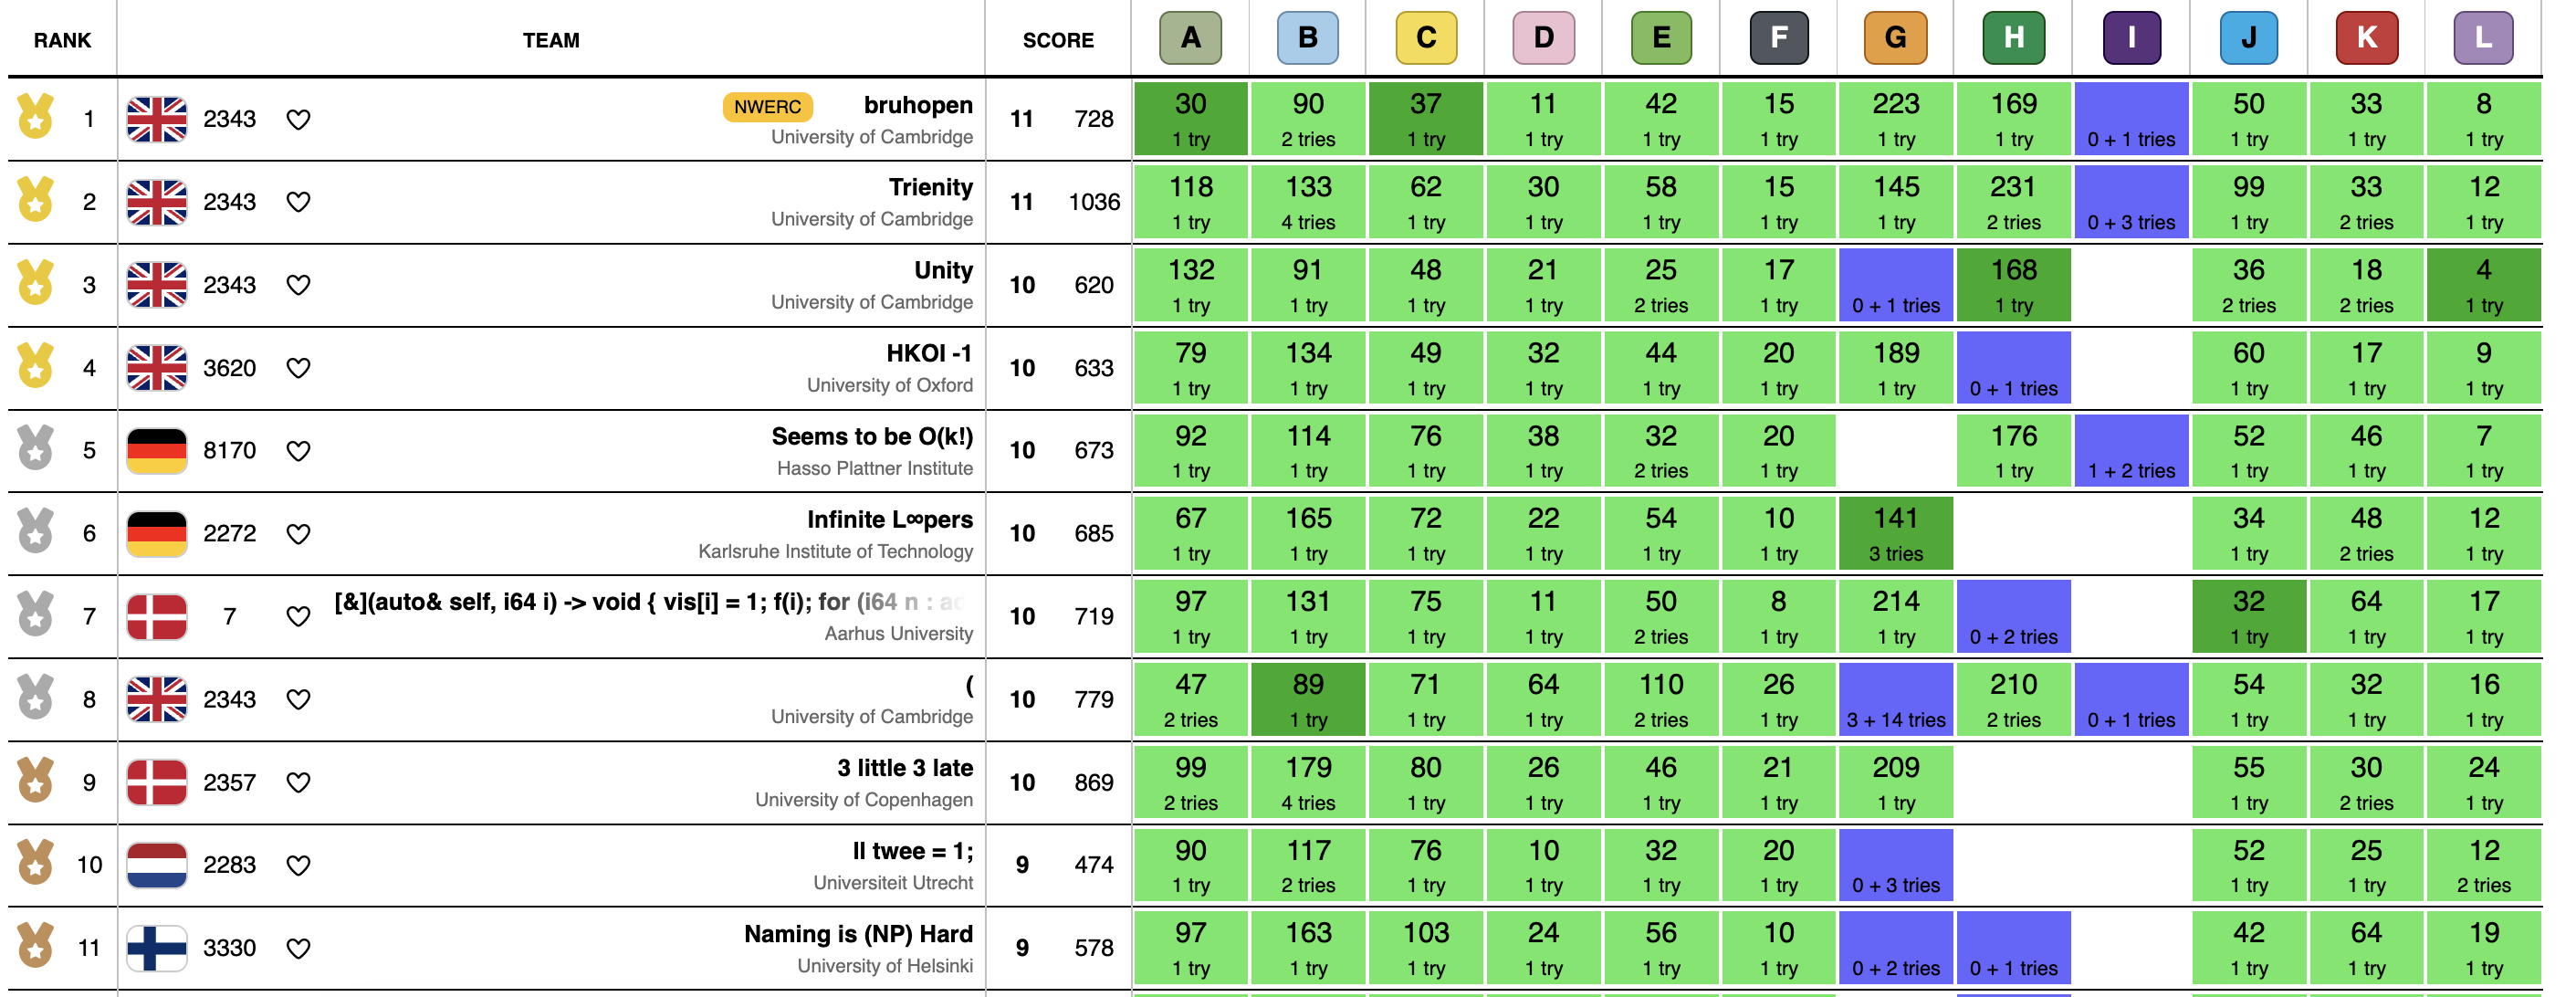
\includegraphics[width=\textwidth]{Imagenes/Vectorial/juez2.png}
  \caption{Interfaz de administración de DOMjudge mostrando el panel de control del concurso, con el estado de los judgehosts y los envíos recientes.}
  \label{fig:juez2}
\end{figure}

\subsection{API REST de DOMjudge}
\label{subsec:domjudge_api}

La funcionalidad más relevante para este trabajo es la API REST de DOMjudge, que expone en formato JSON el estado completo del concurso de forma pública y sin interferir en su funcionamiento. DOMjudge implementa la \textbf{Contest API Specification} de ICPC Tools, un estándar abierto que garantiza la interoperabilidad entre el sistema de jurado y herramientas externas de visualización y retransmisión. La API es accesible en la ruta base \texttt{/api/v4/} del servidor y la mayoría de los endpoints de consulta no requieren autenticación.

La tabla~\ref{tab:domjudge-endpoints} recoge los endpoints más relevantes para la integración con el plugin de RA.

\begin{table}[H]
\centering
\small
\begin{tabularx}{\textwidth}{l l X}
\toprule
\textbf{Método} & \textbf{Endpoint} & \textbf{Descripción} \\
\midrule
GET & \texttt{/contests} & Lista de concursos disponibles, con identificador, nombre y estado. \\[4pt]
GET & \texttt{/contests/\{cid\}/scoreboard} & Marcador completo: posición, problemas resueltos, intentos y penalización de cada equipo. \\[4pt]
GET & \texttt{/contests/\{cid\}/submissions} & Lista de envíos con equipo, problema, lenguaje y marca de tiempo. \\[4pt]
GET & \texttt{/contests/\{cid\}/judgements} & Veredictos asociados a cada envío. \\[4pt]
GET & \texttt{/contests/\{cid\}/teams} & Equipos participantes con nombre, institución y país. \\[4pt]
GET & \texttt{/contests/\{cid\}/problems} & Problemas del concurso con nombre, color del globo y límites. \\
\bottomrule
\end{tabularx}
\caption{Principales endpoints de la API REST de DOMjudge para la integración con el plugin de RA.}
\label{tab:domjudge-endpoints}
\end{table}

A través de estos endpoints, el plugin puede obtener en cada momento la posición de los equipos en el marcador, los veredictos de los envíos más recientes y la información de los equipos y los problemas necesaria para construir los mensajes que se superpondrán en la retransmisión.

DOMjudge proporciona además una documentación interactiva de la API basada en OpenAPI (Swagger UI) accesible en la ruta \texttt{/api/doc} de cualquier instancia. Para el desarrollo y las pruebas del plugin, existe una instancia pública de demostración permanentemente disponible en \url{https://www.domjudge.org/demoweb/}, con datos de un concurso ficticio y la misma API que un servidor real. La documentación interactiva de esa instancia se encuentra en \url{https://www.domjudge.org/demoweb/api/doc}.